\documentclass[a4paper]{article}
\usepackage[a4paper, total={6in, 9.5in}]{geometry} % DL: 쪽여백 조정
\usepackage{setspace} % DL: 줄간격 조정
\usepackage{graphicx} % Required for inserting images
\usepackage{kotex}
\usepackage{amsmath,amsthm,amssymb,amsfonts,mdframed}
\usepackage{tikz}

\renewcommand{\baselinestretch}{1.5}
% \doublespacing % DL: 줄간격 넓혀서
% set indent length to zero.
% \setlength{\parindent}{0pt}

\title{MATH464-01: Combinatorics Term Project Report : Lindström–Gessel–Viennot lemma and its application}
\author{2020160027 박예영}
\date{}
\begin{document}

\maketitle
\section{Motivation}
Lindström–Gessel–Viennot Lemma(LGV lemma)의 증명과 적용에 들어가기에 앞서, 간단한 예시를 통해 Motivation을 잡고자 합니다.\\
다음과 같은 Integer lattice $\mathbb{Z}^2$를 생각해봅시다.\\
\begin{center}
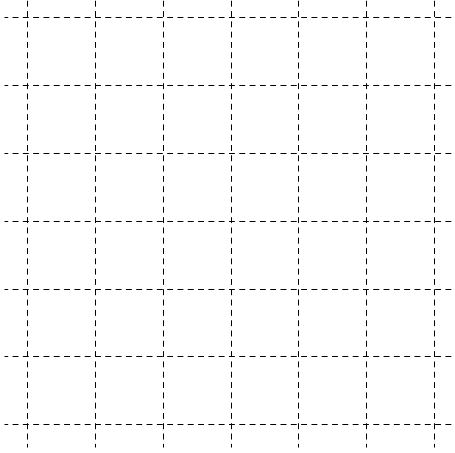
\includegraphics[scale=0.5]{image1.png}
\end{center}
\begin{mdframed}
$\mathbf{DEF)}$ 정점 $u$에서 정점 $v$로 향하는 북동 격자 경로(North-East Lattice Path)(또는 편의 상 격자경로(Lattice Path)라고도 합니다)는 수열 $(v_0, v_1, \cdots, v_n)$로 정의됩니다.\\ 이때, $v_0 = u, v_n = w, v_i \in \mathbb{Z}^2$이고, $v_{i+1} - v_i = (0,1)$ 또는 $(1,0)$을 만족시킵니다.
\end{mdframed}
이 격자 위에 $(0, 0)$에서 $(4, 3)$으로 가는 Lattice Path를 $P_1$, $(1,-1)$에서 $(4,2)$로 가는 Lattice Path를 $P_2$라고 해봅시다.\\
우리는 간단한 조합적 지식을 활용하여 $(0, 0)$에서 $(4, 3)$으로 가는 가능한 모든 Lattice Path $P_1$의 개수를 셀 수 있다는 사실을 알고 있습니다. 이는 $\binom{4+3}{4}$와 같습니다. 마찬가지로, 우리는 가능한 모든 $P_2$의 개수 또한 셀 수 있으며, 이는 $\binom{3+3}{3}$과 같다는 사실을 알고 있습니다.\\
그렇다면, 이 문제를 조금 변형하여, $P_1$과 $P_2$가 공통된 정점을 가지지 않도록 하는, 즉, 경로가 \textbf{교차하지 않도록} 하는 모든 경우의 수는 어떻게 구할까요?\\
단순히 문제를 조금 변형시키기만 했을 뿐인데, 문제가 어려워짐을 확인할 수 있습니다. 이 보고서에서 다루고자 하는 LGV lemma는 이런 상황, 즉, 경로가 교차하지 않도록 하는 경우의 수를 구하는 상황을 효과적으로 계산하는 방법을 제시합니다. 더 나아가, 일반적인 weighted directed acyclic graph에서도 이 문제를 확장시켜 계산할 수 있음을 보여줍니다. LGV lemma는 Schur polynomials의 서로 다른 두 정의가 사실 상 같음을 보여주는 데에도 활용될 수 있으며, The Cauchy–Binet formula를 증명하는데에도 활용됩니다.\\
다시 문제로 돌아와서, $P_1$과 $P_2$가 교차하지 않도록 하는 모든 경우의 수는 어떻게 구할까요? 전체 경우의 수에서 $P_1$과 $P_2$가 교차하는 경우의 수를 빼면 구할 수 있을 것 같습니다.\\
$P_1$과 $P_2$가 교차하는 경우의 수를 구하기 위해, $P_1$과 $P_2$가 특정한 정점에서 교차한다고 생각해봅시다. 그러면, $P_1$과 $P_2$가 만나는 정점들이 있을 것인데, 그 중 사전 순으로 가장 뒤에 있는 정점을 택하고 이를 $c$라고 합시다. (사전 순으로 가장 앞에 있는 정점을 택해도 무방합니다.)\\
\begin{center}
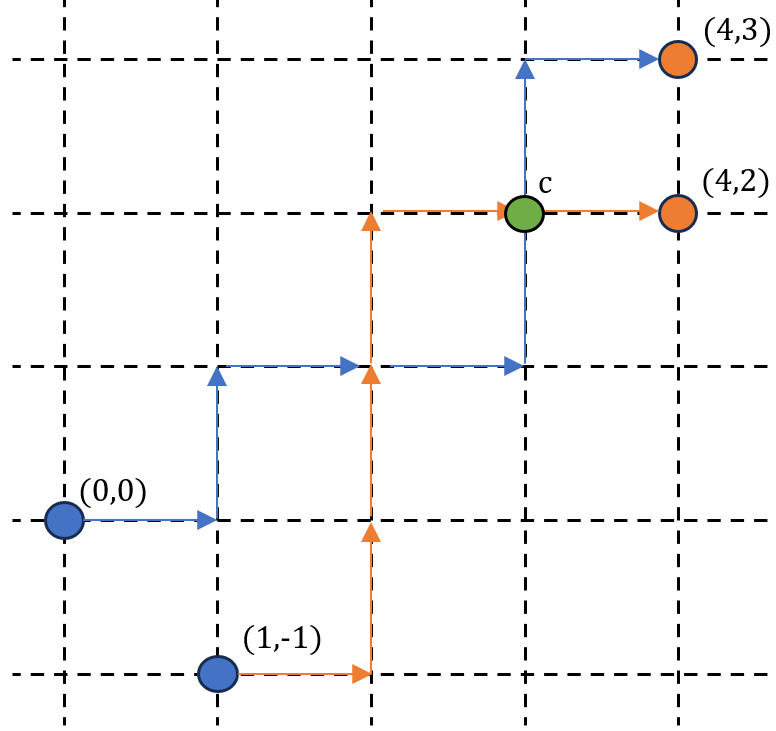
\includegraphics[scale=0.5]{image2.png}
\end{center}
$c$를 기준으로 하여 $P_1$에서 $c$보다 뒤에 있는 정점 $v_i$들을 $P_1$의 tail이라고 하고, 마찬가지로 $P_2$에서 $c$보다 뒤에 있는 정점 $v_i$들을 $P_2$의 tail이라고 한다면, $P_1$의 tail과 $P_2$의 tail을 서로 바꾼 경로 $P_1', P_2'$를 생각할 수 있을 것입니다.\\
즉, $P_1'$은 $(0, 0)$에서 $(4,2)$로 가는 Lattice Path 중 하나이고, $P_2'$은 $(1, -1)$에서 $(4,3)$로 가는 Lattice Path 중 하나입니다. 이때, $(P_1, P_2)$의 개수와 $(P_1', P_2')$의 개수는 자명하게 같음을 확인할 수 있습니다. 왜냐하면 $P_1$과 $P_2$의 tail을 서로 교환하여 만들어진 Path가 $P_1'$과 $P_2'$이기 때문입니다. 또한, $P_1'$과 $P_2'$은 어떤 경로를 그리든 두 경로가 서로 만남을 확인할 수 있습니다.\\
따라서, 가능한 모든 $P_1'$의 개수인 $\binom{4+2}{2}$와 가능한 모든 $P_2'$의 개수인 $\binom{3+4}{3}$을 곱한 $\binom{4+2}{2}\binom{3+4}{3}$가 $P_1$과 $P_2$가 교차하는 경우의 수가 됩니다.\\
전체 경우의 수는 $\binom{4+3}{4}\binom{3+3}{3}$이므로, 우리가 구하고자 하는 답은 $\binom{4+3}{4}\binom{3+3}{3} - \binom{4+2}{2}\binom{3+4}{3}$이 됩니다. 정점 $(0,0), (1, -1)$를 $a_1, a_2$, 정점 $(4,3), (4,2)$를 $b_1, b_2$라고 합시다. 이를 이용하여 위의 식을 다르게 쓰자면 행렬식의 형태와 같이 쓸 수 있습니다.$$\det \begin{pmatrix} \displaystyle \binom{7}{4} & \displaystyle \binom{6}{2}\\[0.3cm] \displaystyle \binom{7}{3} & \displaystyle \binom{6}{3} \end{pmatrix} = \det \begin{pmatrix}
    \textrm{Path }a_1\rightarrow b_1 & \textrm{Path }a_1\rightarrow b_2 \\
    \textrm{Path }a_2\rightarrow b_1& \textrm{Path }a_2\rightarrow b_2
\end{pmatrix}$$
위의 과정을 일반화 한 것이 LGV Lemma입니다.

\newpage
\section{Basic Definitions}
LGV Lemma를 서술하기 위해 필요한 기본 개념들을 알아봅시다.

\begin{mdframed}
\textbf{DEF)} 그래프 $G$는 집합의 쌍 $G = (V,E)$로 정의합니다.\\
이때, $V$는 정점의 집합이며, $E$는 간선의 집합입니다. 간선은 두 정점의 쌍으로 정의합니다.
\end{mdframed}

\begin{mdframed}
\textbf{DEF)} 그래프 $G$의 간선의 집합 $E$에 중복되는 원소가 없으며, $(v, v)$와 같이 같은 정점을 쌍으로 가지고 있는 간선이 존재하지 않은 경우, $G$를 \textbf{단순(simple) 그래프}라고 정의합니다.
\end{mdframed}

\begin{mdframed}
\textbf{DEF)} 그래프 $G$의 간선에 방향이 존재한다면, 즉, $E$의 원소가 두 정점의 쌍으로 정의 되는 것이 아닌, 두 정점의 \textbf{순서쌍}으로 정의된다면, 이 그래프 $G$를 \textbf{유향 그래프(directed graph, digraph)}라고 정의합니다. 
\end{mdframed}

\begin{mdframed}
\textbf{DEF)} \textbf{보행(walk)}은 정점 $v_i$와 간선 $e_i$가 교대로 나타나는 수열 $v_0, e_0, v_1, \cdots, v_k$로 정의합니다. 이때, $e_i = (v_i, v_{i+1})$입니다.
\end{mdframed}

\begin{mdframed}
\textbf{DEF)} 보행(walk)에 나타나는 모든 정점이 서로 다를 경우, 이를 \textbf{경로(path)}라고 정의합니다.
\end{mdframed}

\begin{mdframed}
\textbf{DEF)} 보행(walk)에 나타나는 모든 간선이 서로 다를 경우, 이를 \textbf{트레일(trail)}이라고 정의합니다.
\end{mdframed}

\begin{mdframed}
\textbf{DEF)} 트레일(trail)에 오직 시작 정점과 끝 정점만 같고 나머지 정점들이 모두 서로 다를 경우, 이를 \textbf{사이클(cycle)}이라고 정의합니다.
\end{mdframed}

\begin{mdframed}
\textbf{DEF)} 그래프 $G$에서 만들 수 있는 모든 트레일(trail)이 사이클(cycle)이 아닌 경우, 이 그래프는 \textbf{사이클을 가지고 있지 않다(acyclic)}고 정의합니다.
\end{mdframed}

\begin{mdframed}
\textbf{DEF)} 그래프 $G$의 간선에 방향이 존재하고 사이클을 포함하지 않은 경우, 이 그래프를 \textbf{directed acyclic graph(DAG)}라고 정의합니다.
\end{mdframed}

\begin{mdframed}
\textbf{DEF)} 정점 $v$의 \textbf{차수(degree)}는 다음과 같이 정의합니다. $v$를 쌍의 원소로 가지고 있는 간선을 $e$라고 합시다. 모든 $e$가 가지는 $v$의 개수의 합을 정점 $v$의 차수(degree)라고 정의합니다. 즉, 국소적으로 보았을 때, 정점에 연결되어 있는 간선의 개수를 의미합니다.\\
유향(directed) 그래프의 경우, 정점 $v$의 \textbf{입력 차수(in-degree)}와 \textbf{출력 차수(out-degree)}는 다음과 같이 정의합니다. $v$를 순서쌍의 첫번째 원소로 가지는 간선의 개수를 출력 차수(out-degree), $v$를 순서쌍의 두번째 원소로 가지는 간선의 개수를 입력 차수(in-degree)라고 정의합니다. 즉, 국소적으로 보았을 때, 정점에서 나가는 간선의 개수를 출력 차수, 정점으로 들어오는 간선의 개수를 입력 차수로 정의합니다.
\end{mdframed}

\begin{mdframed}
\textbf{DEF)} 그래프 $G$의 모든 정점의 차수(degree)가 유한할 때, 이 그래프가 \textbf{국소적으로 유한하다(locally finite)}고 정의합니다. 유향 그래프인 경우에는 모든 정점의 입력 차수와 출력 차수가 유한할 때로 정의합니다.
\end{mdframed}

\begin{mdframed}
\textbf{DEF)} 그래프 $G$의 간선 집합 $E$와 임의의 가환환(Commutative Ring) $R$에 대하여, 함수 $W : E \rightarrow R$를 그래프 $G$에 대한 \textbf{가중치 함수(weight function)}이라고 정의합니다. 이 함수를 통해 모든 간선에 가중치(weight)가 부여된 그래프를 \textbf{가중(weighted) 그래프}라고 정의합니다.
\end{mdframed}
LGV Lemma에서 전제하는 그래프 $G$는 사이클이 없고, 국소적으로 유한한 단순 유향 가중 그래프(simple directed weighted acyclic locally finite graph)입니다. 이후에 나오는 모든 개념들은 이를 가정한 상태로 정의하도록 하겠습니다.

\newpage
\section{Statement of LGV Lemma}

그래프 $G$가 위에서 가정한 것과 같은 그래프라고 합시다. 이때 $W$는 그래프의 가중치 함수이며, 위에서 정의한 것처럼 간선의 가중치가 굳이 실수나 정수에 국한될 필요는 없습니다.\\
Motivation을 다시 상기해봅시다. 우리는 \textbf{여러 경로}가 \textbf{서로 교차하지 않도록 하는} 경우의 수를 구하는 문제에서 시작하여, 이를 가중 그래프로 확장하는 작업을 거치고 있습니다. 이에 대한 연장선 상으로, 여러 경로에 대한 개념과 교차하지 않는 것이 무엇인지, 간선의 가중치를 확장한 경로의 가중치에 대한 개념을 생각해봅시다.

\begin{mdframed}
\textbf{DEF)} \textbf{$n$-경로($n$-path)} $P$는 그래프 $G$위의 경로 $P_i$들로 이루어진 $n$-튜플 $(P_1, P_2, \cdots, P_n)$로 정의합니다.
\end{mdframed}

\begin{mdframed}
\textbf{DEF)} 어떤 서로 다른 두 $i, j$에 대하여 $n$-경로($n$-path)의 원소, 즉, 그래프 $G$ 위의 경로 $P_i$와 $P_j$가 서로 공통된 정점을 공유하고 있을 경우, $n$-경로($n$-path)가 \textbf{얽혀있다(entangled)}고 정의합니다. 그렇지 않은 경우 $n$-경로($n$-path)는 \textbf{교차하지 않는다(non-intersecting)}고 정의합니다.
\end{mdframed}
경로의 가중치에 대한 개념을 생각해봅시다.\\[-0.4cm]
\begin{mdframed}
\textbf{DEF)} 경로 $P$에 대한 가중치(weight)는 $P$위의 간선의 가중치의 곱으로 정의하며, 이를 $\omega(P)$라고 표기합니다. 즉, 아래와 같습니다.$$\omega(P) = \prod_{e \in P}W(e)$$
\end{mdframed}
$n$-경로에 대한 가중치 또한 생각해 볼 수 있을 것입니다.\\[-0.4cm]
\begin{mdframed}
\textbf{DEF)} \textbf{$n$-경로($n$-path)} $P$에 대한 가중치(weight)는 $\omega(P_i)$의 곱으로 정의하며, 이를 $\omega(P)$라고 표기합니다. 즉, 아래와 같습니다.$$\omega(P) = \prod_{P_i \in P} \omega(P_i) = \prod_{P_i \in P}\prod_{e \in P_i}W(e)$$
\end{mdframed}
Motivation을 다시 상기해보았을 때, 우리는 행렬식의 형태로 답이 나옴을 알 수 있었습니다. 이때, 각 원소들은 특정 출발 정점과 특정 도착 정점에 대한 경로의 개수였습니다. 이에 대한 연장선 상으로 다음과 같은 개념을 생각해봅시다.\\[-0.4cm]
\begin{mdframed}
\textbf{DEF)} 두 정점 $a$와 $b$에 대하여 $e(a, b)$를 다음과 같이 정의합시다. $$e(a,b) = \sum_{P:a\rightarrow b}\omega(P) = \sum_{P:a\rightarrow b} \prod_{e \in P}W(e)$$ 즉, 정점 $a$에서 정점 $b$로 가는 모든 경로 $P$에 대해, $\omega(P)$의 합입니다. 다시 말해, 정점 $a$에서 정점 $b$로 가는 모든 경로 $P$의 가중치의 합입니다.
\end{mdframed}
만약, 그래프의 모든 간선마다 가중치를 $1$로 부여한다면, $\omega(P)$의 값은 어떤 경로든 상관 없이 $1$로 나오기 때문에 $e(a, b)$의 값은 정점 $a$에서 정점 $b$로 가는 모든 경로의 개수와 같습니다.\\
Motivation에서 확인할 수 있듯이, 우리는 여러 개의 경로들이 겹치지 않도록 하는 경우의 수를 세고자 하는 것이 Lemma의 발단이었습니다. 그리고 이에 대한 답은 행렬식의 형태로 나타남을 확인할 수 있었습니다. 이와 비슷하게, LGV Lemma에서도 비슷한 개념을 생각해봅시다. 이를 정의하기 위해, 그래프 $G$에서 시작 정점과 도착 정점들을 모아놓은 두 정점 집합을 생각합시다. 시작 정점을 모아놓은 집합을 $A = \{a_1, \cdots, a_n\}$이라고 하고, 도착 정점을 모아놓은 집합을 $B = \{b_1, \cdots, b_n\}$이라고 합시다. 이때, 시작 정점 집합과 도착 정점 집합이 서로소(disjoint)일 필요는 없습니다.\\[-0.4cm]
\begin{mdframed}
\textbf{DEF)} 정사각행렬 $M$을 다음과 같이 정의합시다. $$M = \begin{pmatrix}e(a_1,b_1)&e(a_1,b_2)&\cdots&e(a_1, b_n)\\e(a_2, b_1)&e(a_2,b_2)&\cdots&e(a_2,b_n)\\
\vdots&\vdots&\ddots&\vdots\\e(a_n,b_1)&e(a_n,b_2)&\cdots&e(a_n,b_n)\end{pmatrix}$$
이 행렬을 $A$에서 $B$로 가는 경로 행렬(path matrix)이라고 부릅니다. 경로 행렬 $M$의 $i$번째 행, $j$번째 열에 놓인 원소 $M_{ij}$는 $e(a_i,b_j)$입니다.
\end{mdframed}

\begin{mdframed}
\textbf{DEF)} 기존의 $n$-경로 $P$의 원소가 $P_i : a_i \rightarrow b_i$로 주어져 있다고 합시다. 즉, $a_i$에서 $b_i$로 가는 경로가 $P_i$라고 해봅시다. \textbf{뒤틀린 $n$-경로(Twisted $n$-path) $P'$}는 기존의 $n$-경로 $P$가 주어져 있을 때, 대칭군(symmetric group) $S_n$의 원소 $\sigma$, 즉, 어떤 순열(permutation) $\sigma$에 대해서, $(a_1, a_2, \cdots, a_n)$에서 $(b_{\sigma(1)}, b_{\sigma(2)}, \cdots, b_{\sigma(n)})$로 가는 새로운 $n$-경로 $P'$로 정의합니다. 이때, $\sigma$는 $n$-경로 $P$의 \textbf{뒤틀림(twist)}이라고 정의합니다.\\
다시 말해, 기존의 $n$-경로 $P$가 시작 정점 $a_i$에서 도착 정점 $b_i$로 가는 $P_i$들의 튜플이었다면, 뒤틀린 $n$-경로 $P'$은 시작 정점 $a_i$에서 도착 정점 $b_{\sigma(i)}$로 가는 $P_i$들의 튜플입니다.\\
$\mathrm{sgn}(P') = \mathrm{sgn}(\sigma)$로 정의합니다. 
\end{mdframed}
시작 정점 집합 $A$에서 도착 정점 집합 $B$로 향하는 모든 $n$-경로 $P$들을 생각해봅시다. 이때, 어떤 순열 $\sigma$가 존재하여, $n$-경로의 원소 $P_i$는  시작 정점이 $a_i$이고, 도착 정점이 $b_{\sigma(i)}$인 경로입니다. 즉, $n$-경로 $P$의 모든 도착 정점들의 집합은 $B$입니다.\\
이 상황에서, 모든 교차하지 않는 $n$-경로의 집합을 $NI$, 모든 얽혀있는 $n$-경로의 집합을 $ET$라고 합시다. 또한, $A$에서 $B$로 가는 경로 행렬을 $M$이라고 합시다. 이때, LGV Lemma는 다음과 같습니다. $$\det(M) =  \sum_{P \in NI}\mathrm{sgn}(P)\omega(P)$$
즉, LGV Lemma는 경로 행렬의 행렬식의 값이 모든 교차하지 않는 $n$-경로의 부호있는 가중치의 합과 같음을 이야기 해줍니다. 특히, 만약 그래프의 모든 가중치가 $1$이고 교차하지 않도록 만드는 뒤틀림 $\sigma$가 오직 항등 함수 $\mathrm{id}$만 존재한다면, 이 행렬 식의 값은 시작 정점 집합 $A$에서 도착 정점 집합 $B$로 향하는 교차하지 않는 모든 $n$-경로의 개수와 같습니다. 다시 말해, 이 상황은 위에서 제시한 Motivation의 상황과 동일한 상황이 됩니다.\\

\section{Proof of LGV Lemma}
행렬식 $\det(M)$에 대한 정의를 생각해봅시다. $$\det(M) = \sum_{\sigma \in S_n} \mathrm{sgn}(\sigma)\prod_{i=1}^{n}e(a_i, b_{\sigma(i)})$$ 뒷부분만 따로 생각해봅시다. $$\mathrm{sgn}(\sigma)\prod_{i=1}^{n}e(a_i, b_{\sigma(i)}) = \mathrm{sgn}(\sigma)e(a_1, b_{\sigma(1)})e(a_2, b_{\sigma(2)})\cdots e(a_n, b_{\sigma(n)})$$ 이때, $e(a_i, b_{\sigma(i)})$는 위의 정의에 따라 $a_i$에서 $b_{\sigma(i)}$로 가는 모든 경로 $P_i$의 가중치의 합입니다. 이를 모든 $P_i$에 대해서 곱했으므로, $n$-경로 $P = (P_1, P_2, \cdots, P_n)$로 표현하여 다음과 같이 쓸 수 있습니다.
\begin{eqnarray*} \mathrm{sgn}(\sigma)e(a_1, b_{\sigma(1)})e(a_2, b_{\sigma(2)})\cdots e(a_n, b_{\sigma(n)}) \\
= \mathrm{sgn}(\sigma)  \sum_{\substack{P : (a_1, \cdots, a_n)\\ \downarrow \\(b_{\sigma(1)}, \cdots, b_{\sigma(n)})}} \omega(P) \\
=  \sum_{\substack{P : (a_1, \cdots, a_n)\\ \downarrow \\(b_{\sigma(1)}, \cdots, b_{\sigma(n)})}} \mathrm{sgn}(P) \omega(P)
\end{eqnarray*}
따라서, 행렬식 $\det(M)$을 아래와 같이 이중 합으로 표현할 수 있습니다.
\begin{eqnarray*} \det(M) = \sum_{\sigma \in S_n} \sum_{\substack{P : (a_1, \cdots, a_n)\\ \downarrow \\(b_{\sigma(1)}, \cdots, b_{\sigma(n)})}} \mathrm{sgn}(P) \omega(P)
\end{eqnarray*}
어떤 뒤틀림 $\sigma$가 정해지면 이에 대한 모든 $n$-경로의 부호있는 가중치의 합이 계산되므로, 우리는 행렬식의 값이 시작 정점의 집합 $A$에서 도착 정점의 집합 $B$로 가는 모든 $n$-경로들의 부호있는 가중치의 합임을 알 수 있습니다. 즉, 다음과 같습니다. $$\det(M) = \sum_{P:A \rightarrow B} \mathrm{sgn}(P)\omega(P)$$
우리는 이전에 $A$에서 $B$로 가는 모든 $n$-경로들을 두가지 부류로 나눴습니다. $n$-경로는 교차하지 않는 $n$-경로의 집합인 $NI$에 속하거나, 얽혀있는 $n$-경로의 집합인 $ET$에 속하므로 위의 식을 다음과 같이 다시 작성할 수 있습니다. $$\det(M) = \sum_{P \in NI} \mathrm{sgn}(P)\omega(P) + \underbrace{\sum_{P \in ET} \mathrm{sgn}(P)\omega(P)}_{\textrm{have to be 0}}$$
따라서, 우리는 $ET$에 속하는 모든 $n$-경로 $P$의 부호있는 가중치의 합이 $0$임을 보여주면 됩니다.\\
이를 위해, $\omega(f(P)) = \omega(P)$이고, $\mathrm{sgn}(f(P)) = -\mathrm{sgn}(P)$를 만족시키는 대합(involution) $f : ET \rightarrow ET$를 구성해봅시다. 이러한 대합이 만들어진다면, $ET$에 속하는 어떠한 $n$-경로 $P$는 이에 대응되는 $f(P)$가 있어서, $\mathrm{sgn}(P)\omega(P) + \mathrm{sgn}(f(P))\omega(f(P)) = 0$을 만족시키기 때문에 뒤의 식이 $0$임을 보여줄 수 있습니다.\\
\begin{center}
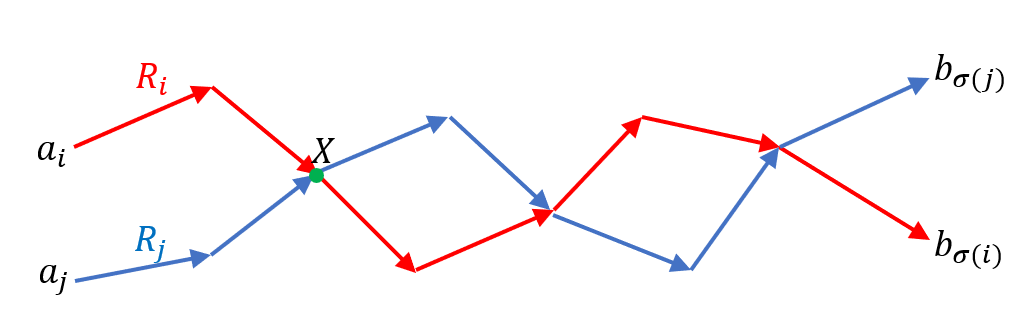
\includegraphics[scale=0.6]{image3.png}
\end{center}
$R = (R_1, R_2, \cdots, R_n) \in ET$를 생각해봅시다. $R$은 얽혀있는 $n$-경로이기 때문에, 어떤 특정한 두 경로 $R_i$와 $R_j$가 서로 같은 정점을 공유하고 있을 것입니다. 좀 더 명확한 진술을 위해 아래와 같이 정의합시다.
\begin{itemize}
    \item $(i, j)$는 $x \neq y$이며 $R_x$와 $R_y$가 서로 같은 정점을 공유하고 있을 때, 이러한 순서쌍 $(x, y)$ 중에서 사전 순으로 가장 작은 순서쌍입니다.
    \item $X$는 $R_i$와 $R_j$가 공유하는 첫번째 정점입니다.
    \item $L_{iX}$, $R_{iX}$는 $X$를 기준으로 왼쪽과 오른쪽으로 분리된 $R_i$의 부분 경로를 의미합니다. 즉, $L_{iX}$는 $a_i$에서 $X$로 향하는 $R_i$의 일부분을, $R_{iX}$는 $X$에서 $b_{\sigma(i)}$로 향하는 $R_i$의 일부분을 뜻합니다.
    \item 마찬가지로, $L_{jX}$, $R_{jX}$는 $X$를 기준으로 왼쪽과 오른쪽으로 분리된 $R_j$의 부분 경로를 의미합니다.
\end{itemize}
\begin{center}
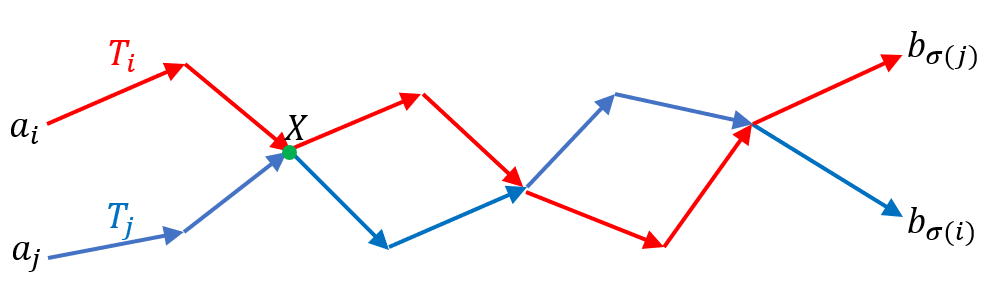
\includegraphics[scale=0.6]{image4.png}
\end{center}
이때 $R$에 대응되는 $T = (T_1, T_2, \cdots, T_n) \in ET$를 생각해봅시다. 이 $T$는 위에서 언급한 $R_i$와 $R_j$의 뒷부분만 서로 교환한 새로운 $n$-경로입니다. 명확한 진술을 위해, 아래와 같이 정의합시다.
\begin{itemize}
    \item $k \neq i,j$인 경우, $T_k$ = $R_k$입니다.
    \item $T_i$는 경로 $L_{iX}$와 $R_{jX}$를 이은 경로입니다.
    \item $T_j$는 경로 $L_{jX}$와 $R_{iX}$를 이은 경로입니다.
\end{itemize}
$n$-경로 $T$는 단순히 $n$-경로 $R$의 간선만을 사용하여 만들어진 경로이기 때문에, $\omega(T) = \omega(R)$임은 자명합니다. 또한, 이렇게 만들어진 $T$는 $R$과 유일하게 대응됨 또한 확인할 수 있습니다. 또한, $T$가 가지는 뒤틀림을 $\sigma'$이라고 한다면, $T_i$과 $T_j$의 도착 정점은 오직 $R_i$와 $R_j$의 도착 정점만 서로 뒤바꾼 상태이기 때문에 $\sigma' = \sigma \circ (i, j)$가 성립합니다. 따라서, $\mathrm{sgn}(T) = \mathrm{sgn}(\sigma') = \mathrm{sgn}(\sigma \circ (i, j)) = - \mathrm{sgn}(\sigma) = - \mathrm{sgn}(R)$이 성립합니다.\\
따라서 대합(inversion) $f : ET \rightarrow ET$를 어떠한 $n$-경로$R$에 대해서, 이러한 $T$로 대응되도록 하는 대합으로 정의하면 충분합니다. 이로써 증명이 완료되었습니다.

\newpage
\section{Application of LGV Lemma}
\begin{mdframed}
\textbf{THM)} (Cauchy–Binet formula)\\
모든 두 $n\times n$ 행렬 $M_1$, $M_2$에 대하여 다음과 같은 식이 성립합니다.$$\det(M_1M_2) = \det(M_1)\det(M_2)$$
\end{mdframed}
\begin{proof}
간단한 행렬식의 성질이긴 하지만, 우리는 이를 LGV Lemma의 관점에서도 증명할 수 있습니다. 먼저, 아래와 같은 정점 집합을 생각해봅시다.
\begin{eqnarray*}
A = \{a_1, a_2, \cdots, a_n\}\\
B = \{b_1, b_2, \cdots, b_n\}\\
C = \{c_1, c_2, \cdots, c_n\}
\end{eqnarray*}
이제, $M_1$을 $A$에서 $B$로 향하는 경로 행렬이라고 정의하고, $M_2$를 $B$에서 $C$로 향하는 경로 행렬이라고 정의합시다. 그러면 $M = M_1M_2$의 원소는 $$M_{ik} = \sum_{j=1}^n e(a_i,b_j)e(b_j,c_k)$$임을 알고 있습니다.\\
$A$에서 $C$로 향하는 교차하지 않는 $n$-경로를 $P$라고 한다면, $P$는 반드시 $B$를 거칠 수 밖에 없습니다. 우리는 $B$를 기준으로 하여 $P$의 경로를 $Q$와 $R$로 \textbf{분리할 수 있습니다}. $A$에서 $B$로 향하는 교차하지 않는 $n$-경로의 집합을 $W$, $B$에서 $C$로 향하는 교차하지 않는 $n$-경로의 집합을 $Z$라고 한다면, $Q$와 $R$은 각각 $W$와 $Z$에 속함을 명백하게 알 수 있습니다. 따라서 다음과 같은 식이 성립합니다.
\begin{eqnarray*}
\det(M_1)\det(M_2)\\ = \sum_{Q \in W}\mathrm{sgn}(Q)\omega(Q) \sum_{R \in Z}\mathrm{sgn}(R)\omega(R)\\
= \sum_{P \in W\times Z}\mathrm{sgn}(R)\mathrm{sgn}(Q)\omega(R)\omega(Q)\\
= \sum_{P}\mathrm{sgn}(P)\omega(P)\\
= \det(M_1M_2)
\end{eqnarray*}
\end{proof}
\begin{mdframed}
\textbf{Problem)} 모든 $m, n \in \mathbb{N}$에 대하여 다음과 같은 식이 성립합니다.
$$
\begin{vmatrix}
\binom{m}{0} & \binom{m}{1} & \cdots & \binom{m}{n-1} \\
\binom{m+1}{0} & \binom{m+1}{1} & \cdots & \binom{m+1}{n-1} \\
\vdots & \vdots & \ddots & \vdots \\
\binom{m+n-1}{0} & \binom{m+n-1}{1} & \cdots & \binom{m+n-1}{n-1} \\
\end{vmatrix} = 1
$$
\end{mdframed}
\begin{proof}
위의 행렬식을 LGV Lemma에서 사용되는 행렬식이라고 생각해봅시다. 즉, 행렬의 원소가 $A_i$에서 $B_j$로 가는 경로들의 가중치의 합이라고 생각합시다. 형태를 보면 익숙하겠지만, 이항 계수의 형태로 나타나있기 때문에, 우리는 가중치가 모두 1로 통일되어있는 격자 경로의 모습을 생각해 볼 수 있습니다.
\begin{center}
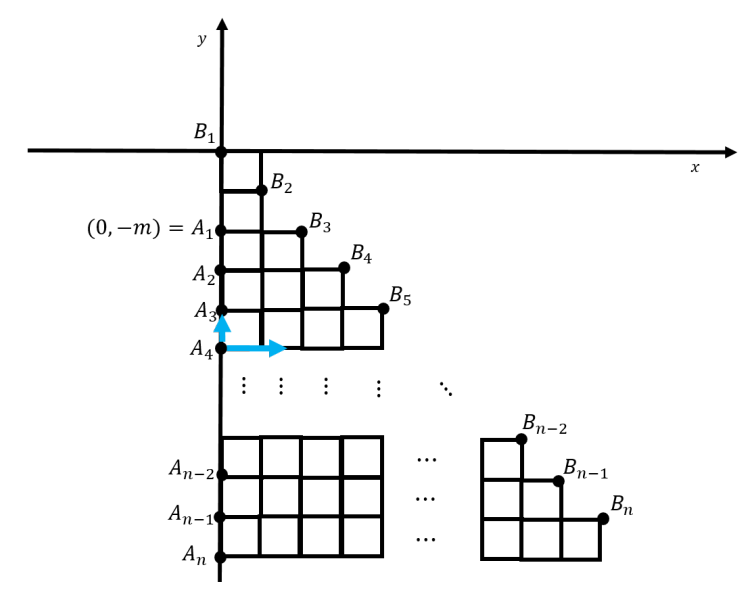
\includegraphics[scale=0.6]{image5.png}
\end{center}
즉, 다음과 같은 격자 경로의 모습을 생각할 수 있습니다. 이제, $(A_1, \cdots, A_n)$에서 $(B_1, \cdots, B_n)$로 가는 교차하지 않는 $n$-경로의 개수를 생각해봅시다. $A_1$에서 $B_1$로 가는 경로는 오직 하나밖에 존재하지 않습니다. $A_2$에서 $B_2$로 가는 경로는 위의 경로와 겹치지 않아야 하므로, 무조건 처음에는 오른쪽으로 한 칸을 가야 합니다. 따라서 겹치지 않도록 하는 조건을 만족시키기 위한 경우의 수는 $1$가지 밖에 없습니다. 마찬가지로, $A_i$에서 $B_i$로 향하는, 겹치지 않는 경우의 수는 이전 경로들에 의해 오직 한 가지로 밖에 정해지지 않으므로, 위의 행렬식은 $1$의 값이 나옴을 확인할 수 있습니다. 
\end{proof}

\section{Conclusion}
이 이외에도, LGV Lemma는 다양한 조합론 분야에 활용될 수 있습니다. 여기서 소개하지는 않았지만, Schur polynomials와 관련이 있어, hook's length formula와도 관련이 있고, 위의 예시들처럼 행렬에 대한 문제를 가중 그래프에 관한 문제로 끌고 와서 해결하는 방안을 제시하기도 합니다. 대표적으로는 Motivation에서 언급한 것처럼, 격자 경로 위에서의 경우의 수를 세는 문제 또한 이 Lemma를 이용하여 해결할 수 있습니다.\\

\section*{References}
\begin{enumerate}
    \item Gessel, Ira M.; Viennot, Xavier G. (1989), Determinants, Paths and Plane Partitions
    \item Martin, Jeremy (2012), Lecture Notes on Algebraic Combinatorics
    \item Fulmek, Markus (2010), Viewing determinants as nonintersecting lattice paths yields classical determinantal identities bijectively, arXiv:1010.3860v1
    \item Edin Lidan, Lindström–Gessel–Viennot theorem as a common point of linear algebra and combinatorics
    \item Miaowtin, Lattice paths and Lindström–Gessel–Viennot lemma,\\ https://codeforces.com/blog/entry/108395
    \item Rui Xiong, Schur Polynomials through Lindström Gessel Viennot Lemma, arXiv:2003.09215
    \item Jang Soo Kim, [Topics in Combinatorics] Lecture 9. Gessel Viennot Lindstrom lemma,\\
 https://youtu.be/DqmtJwNhIeU?si=GIBrQtTDEdRfDTGT
\end{enumerate}
\end{document}
